% Requires: \usepackage{graphicx, subcaption}
\begin{figure}[t]
  \centering
  \begin{subfigure}[t]{0.48\textwidth}
    \centering
    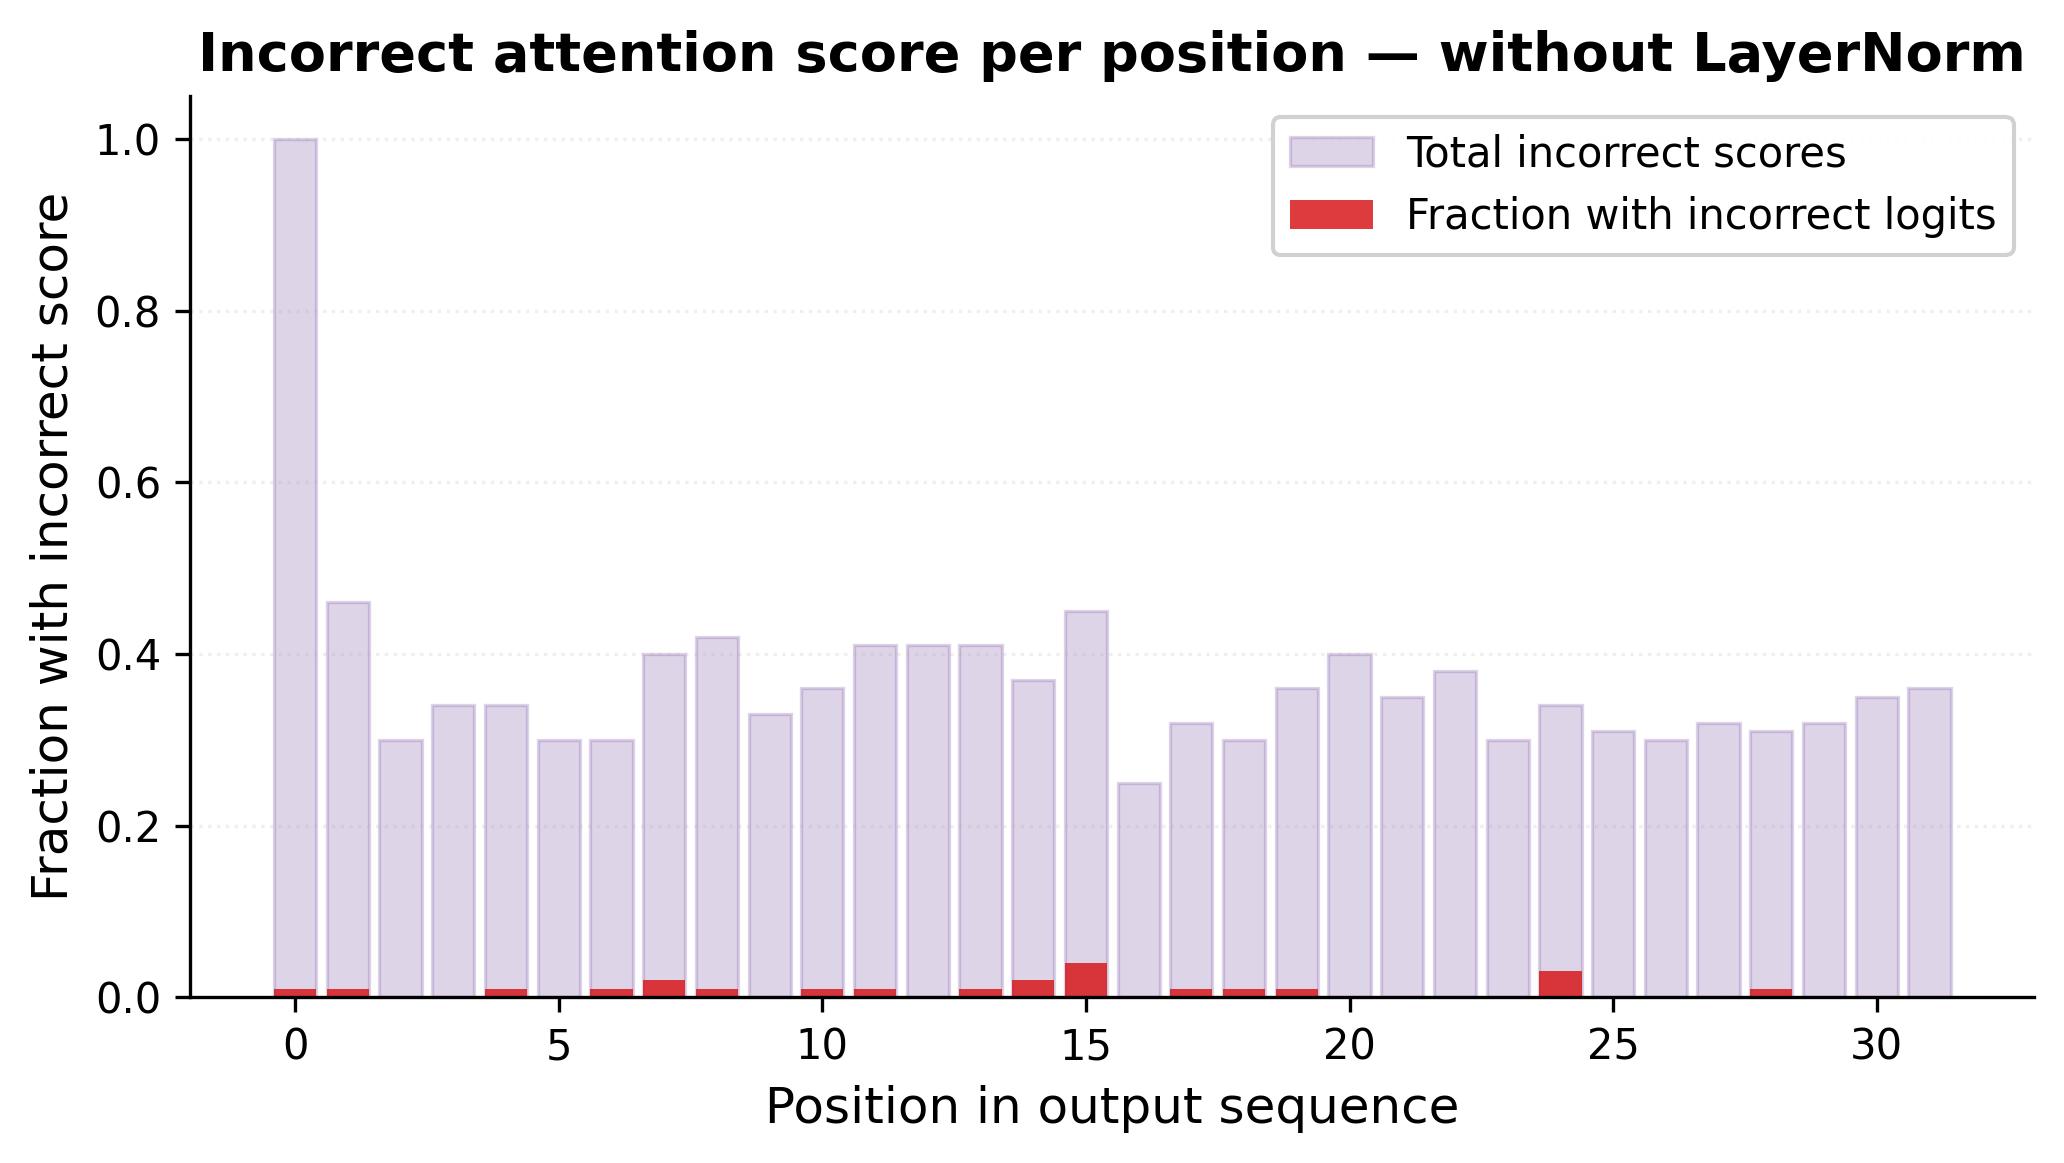
\includegraphics[width=\linewidth]{results/attention_errors/icscore_perlocation.png}
    \label{fig:icscore_perlocation}
  \end{subfigure}
  \hfill
  \begin{subfigure}[t]{0.48\textwidth}
    \centering
    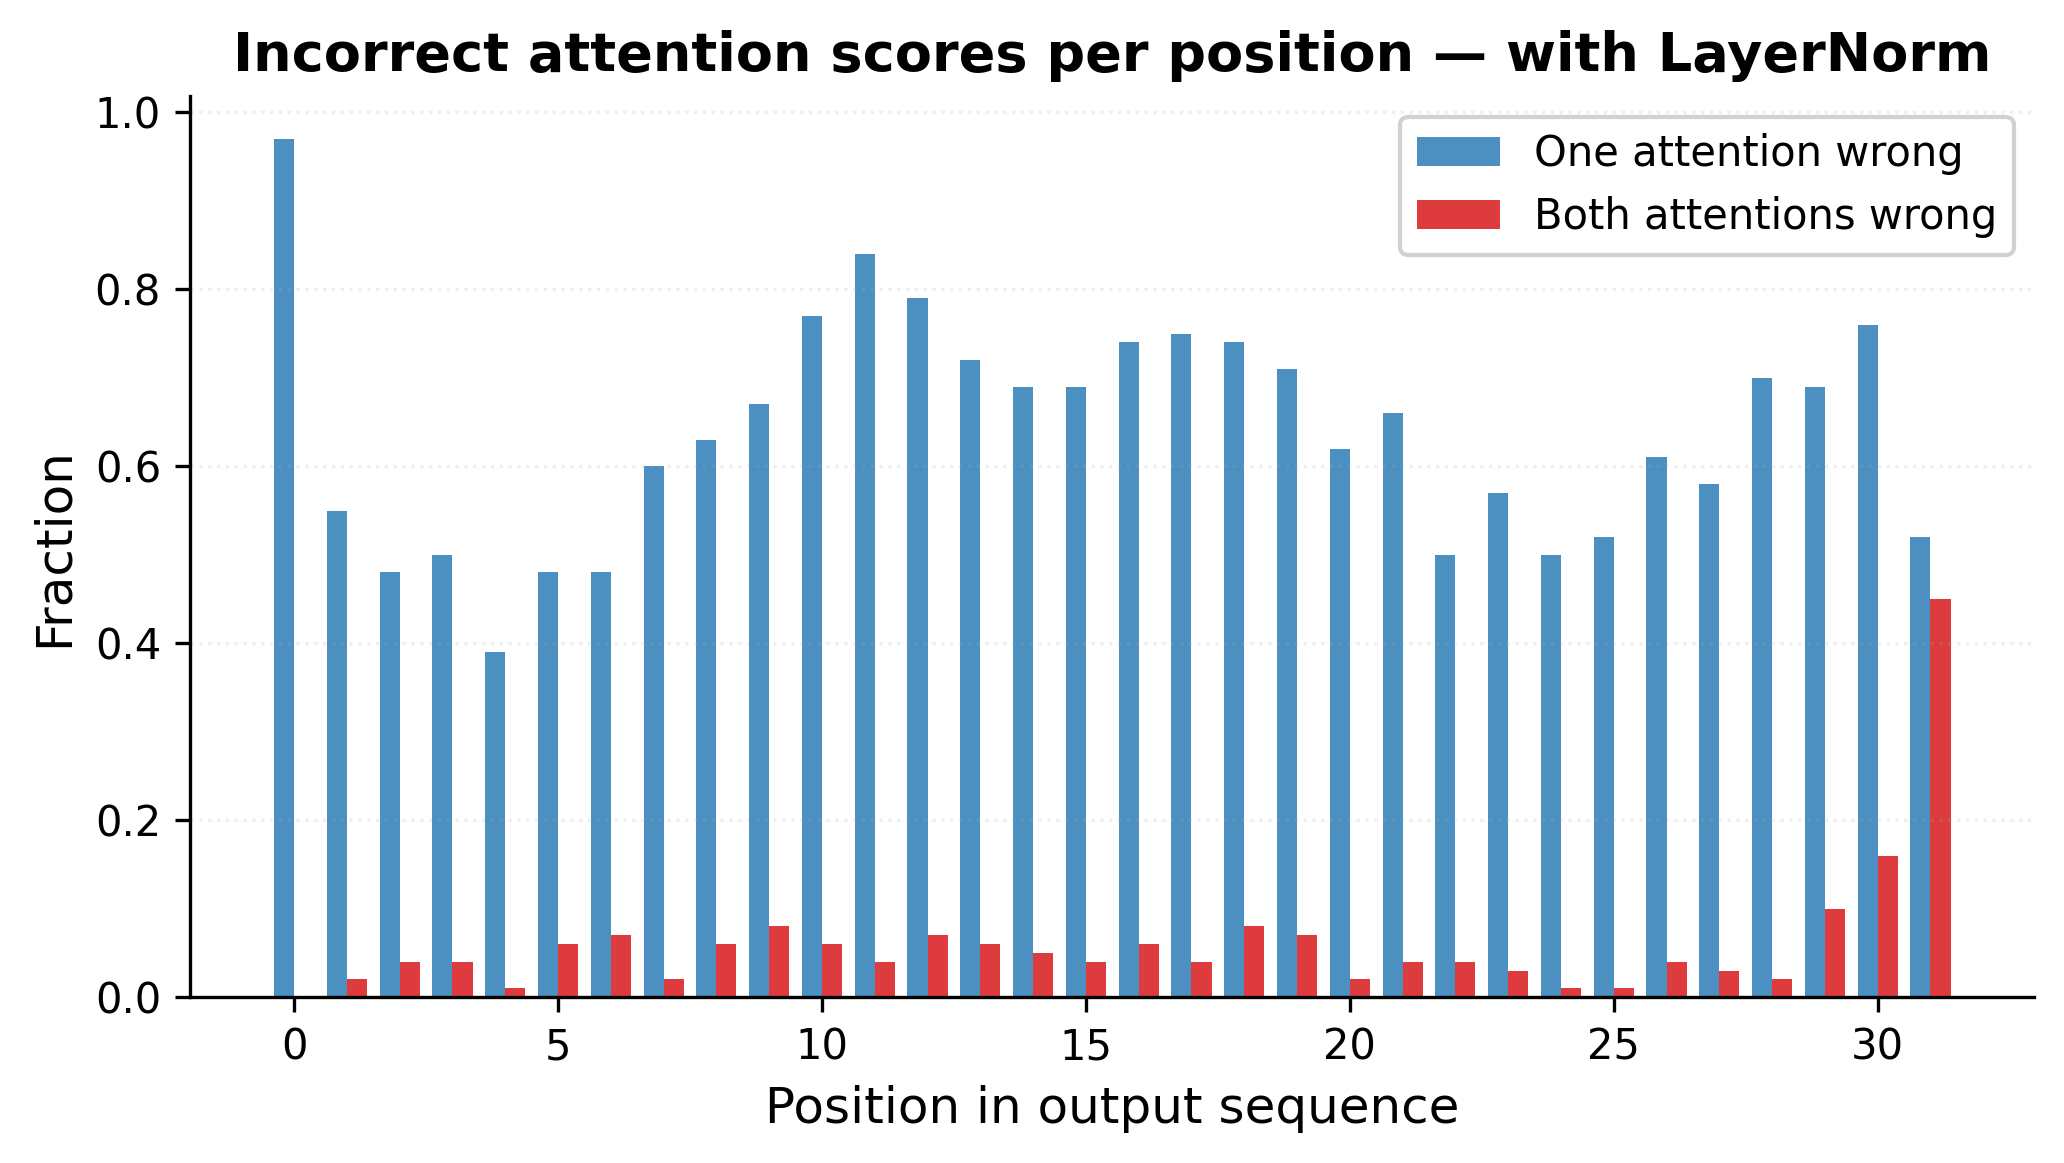
\includegraphics[width=\linewidth]{results/attention_errors/correction_fraction_withlayernorm.png}
    \label{fig:correction_fraction_withln}
  \end{subfigure}
  \caption{Per-position analysis of incorrect attention scores. \textbf{(Left)}~Fraction of incorrect first-layer attention scores for the model without layer normalization, decomposed into cases where the final logit is correct (total transparent bar) versus incorrect (solid red). \textbf{(Right)}~Fraction of incorrect attention scores across both layers for the model with layer normalization, showing cases where exactly one or both layers spike on the wrong token.}
  \label{fig:attention_errors}
\end{figure}
